\chapter{Собственное расстояние, геометрия Крускала и наблюдатели у горизонта}

Метрика Шварцшильда кажется сингулярной на горизонте. Кривизна — нет. Чтобы отделить одно от другого, мы сначала выносим общий масштаб черной дыры, а затем заменяем радиальную координату собственным расстоянием от горизонта. Вблизи горизонта получающаяся геометрия — это обычное плоское пространство-время, записанное в ускоренных координатах. Как только эта геометрия нарисована, вопросы об Алисе, Бобе и Чарли становятся вопросами о мировых линиях и световых лучах, а не словесными парадоксами.

\section{Выделение радиуса Шварцшильда как общего масштаба}

Начнем со штрихованных координат, чтобы масштабированные переменные позже могли получить привычные имена:
\begin{equation}
d\tau^2
=
\left(1-\frac{2MG}{r'}\right)dt'^2
-
\frac{dr'^2}{1-\frac{2MG}{r'}}
-
r'^2d\Omega_2^2.
\label{eq:l7-schwarzschild-dimensional}
\end{equation}
Введем радиус Шварцшильда и безразмерные координаты
\begin{equation}
r_{\mathrm S}=2MG,
\qquad
r=\frac{r'}{r_{\mathrm S}},
\qquad
t=\frac{t'}{r_{\mathrm S}}.
\label{eq:l7-rescaling}
\end{equation}
Мы используем \(c=1\), поэтому время и длина имеют одинаковые единицы. Следовательно, радиус
\(r_{\mathrm S}\) является и длиной, и связанным с этой длиной временем прохождения света. Подстановка дает
\begin{equation}
d\tau^2
=r_{\mathrm S}^2
\left[
\left(1-\frac1r\right)dt^2
-
\frac{dr^2}{1-\frac1r}
-
r^2d\Omega_2^2
\right].
\label{eq:l7-schwarzschild-rescaled}
\end{equation}
Следовательно, все невращающиеся незаряженные черные дыры Шварцшильда имеют одну и ту же безразмерную геометрию. Изменение массы меняет линейку, умножающую метрику, а не форму выражения в скобках. Ситуация похожа на изображение сфер после деления каждого расстояния на радиус сферы: один и тот же рисунок описывает Луну и Землю, хотя сантиметр на одном рисунке соответствует другому физическому расстоянию.

\begin{classroomqa}
\audiencequestion{Какие знаки должны стоять у радиальной и угловой частей метрики?}
\lecturerresponse{При используемой здесь сигнатуре \(+---\) обе пространственные части идут со знаками минус. Аудитория заметила ошибку со знаком, пока выражение записывалось. Угловой множитель может содержать синус или косинус в зависимости от того, отсчитывается ли полярная координата от оси или от экватора; компактное обозначение \(d\Omega_2^2\) позволяет избежать этой зависимости от соглашения.
\lecturetimestamp{00:07:48--00:08:12}}
\end{classroomqa}

\section{Масштаб кривизны на горизонте}

Масштабирование отвечает на важный физический вопрос без длинного тензорного вычисления. Компонента метрики безразмерна. Символ Кристоффеля содержит одну производную по координате и потому имеет размерность обратной длины, тогда как компонента тензора Римана в физическом ортонормированном базисе имеет размерность
\begin{equation}
[g_{\mu\nu}]=1,
\qquad
[\Gamma^\mu{}_{\nu\rho}]=L^{-1},
\qquad
[R_{\hat\alpha\hat\beta\hat\gamma\hat\delta}]
=L^{-2}.
\label{eq:l7-curvature-dimensions}
\end{equation}
На горизонте \(r=1\) единственная доступная физическая длина —
\(r_{\mathrm S}\). Следовательно, масштаб приливной кривизны должен быть
\begin{equation}
\left|R_{\hat\alpha\hat\beta\hat\gamma\hat\delta}\right|_{\mathrm{hor}}
\sim \frac{1}{r_{\mathrm S}^2}.
\label{eq:l7-horizon-curvature}
\end{equation}
Вообще говоря, это \(r_{\mathrm S}^{-2}\), умноженное на безразмерную функцию от
\(r\). Это утверждение относится к приливному полю Римана, а не к скаляру Риччи, который в вакууме Шварцшильда обращается в нуль.

Физический вывод непосредственен. Увеличение массы увеличивает
\(r_{\mathrm S}\) и ослабляет приливное поле на горизонте. Маленькая черная дыра может разорвать протяженное тело при пересечении; у горизонта сверхмассивной черной дыры приливные силы могут быть слабыми. Тем не менее по мере движения внутрь кривизна растет и расходится при \(r=0\). Следовательно, горизонт и сингулярность — радикально разные объекты.

\section{Собственное расстояние от горизонта}

Для остальной части локального вычисления положим \(r_{\mathrm S}=1\). В теории относительности замены координат — не косметика: неудачная координата может скрыть регулярную геометрию за сингулярными коэффициентами. Разность шварцшильдовской координаты \(r-1\) не является измеряемым радиальным расстоянием от горизонта.

\begin{figure}[htbp]
\centering
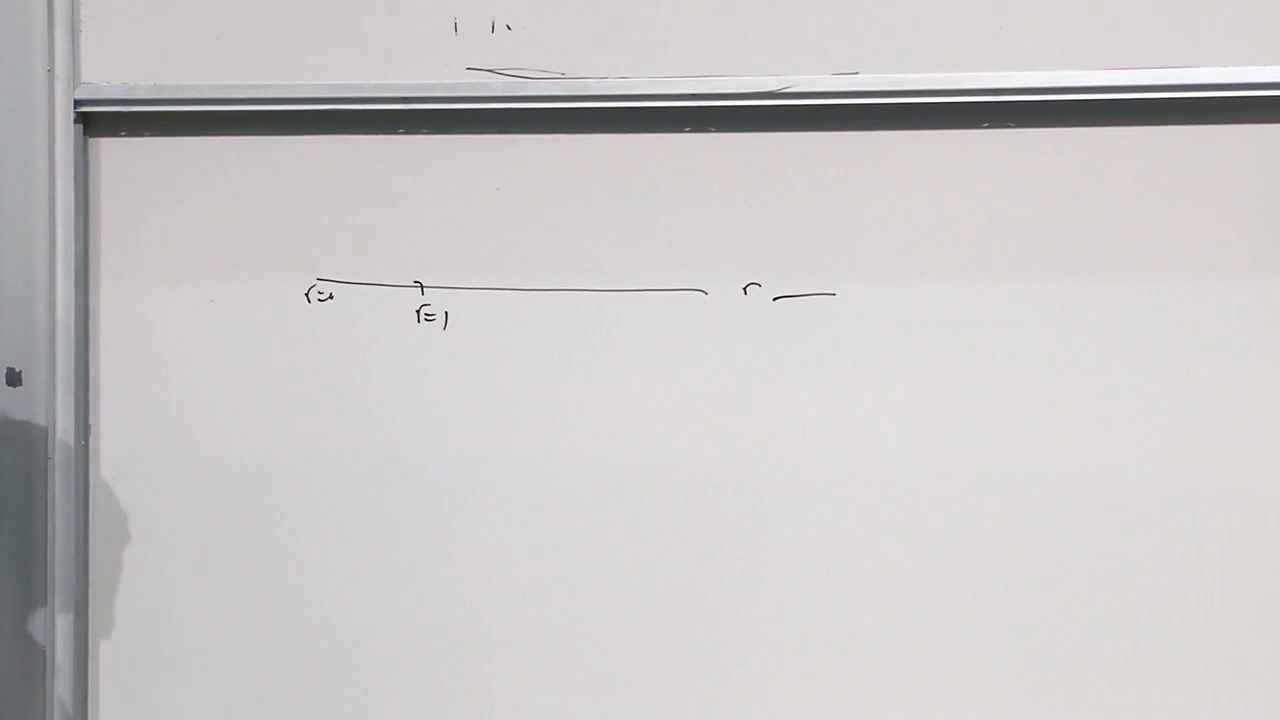
\includegraphics[width=0.78\textwidth]{lecture_07_figure_02.png}
\caption{Радиальная координатная прямая, использовавшаяся на доске. Горизонт находится при
\(r=1\), тогда как \(r=0\) — сингулярность кривизны.}
\lectureframe{00:16:11}
\end{figure}

Зафиксируем \(t\) и углы. Тогда положительный пространственный элемент длины равен
\begin{equation}
ds^2=\frac{dr^2}{1-\frac1r},
\qquad
ds=\sqrt{\frac{r}{r-1}}\,dr.
\label{eq:l7-radial-proper-line}
\end{equation}
Определим безразмерное собственное расстояние от горизонта как
\begin{equation}
\rho(r)
=
\int_1^r\sqrt{\frac{r'}{r'-1}}\,dr'.
\label{eq:l7-rho-definition}
\end{equation}
При восстановлении общего масштаба физическое расстояние равно \(r_{\mathrm S}\rho\). Замкнутая форма интеграла нам не понадобится. Нам нужна только его производная:
\begin{equation}
\frac{d\rho}{dr}
=\sqrt{\frac{r}{r-1}},
\qquad
d\rho^2
=\frac{dr^2}{1-\frac1r}.
\label{eq:l7-rho-derivative}
\end{equation}
Таким образом, сложный радиальный член в точности превращается в \(-d\rho^2\). Именно ради этого упрощения и вводится \(\rho\).

Теперь еще раз масштабируем временную координату,
\begin{equation}
\omega=\frac{t}{2}.
\label{eq:l7-omega}
\end{equation}
Поскольку \(r\) является функцией \(\rho\), метрику можно записать в виде
\begin{equation}
d\tau^2
=
F(\rho)\rho^2d\omega^2
-
d\rho^2
-
r(\rho)^2d\Omega_2^2.
\label{eq:l7-rho-metric}
\end{equation}

\begin{classroomqa}
\audiencequestion{Не определяется ли \(F(\rho)\) просто так, чтобы коэффициент при времени имел вид \(F(\rho)\rho^2\)?}
\lecturerresponse{Да. На этом этапе такая факторизация не имеет самостоятельного физического содержания. Это удобное определение. Ее полезность проявляется, когда рассматривают пределы \(F\) вблизи горизонта и вдали от него.
\lecturetimestamp{00:26:39--00:26:59}}
\end{classroomqa}

Вдали временной коэффициент метрики Шварцшильда стремится к единице. Поскольку
\(dt=2d\omega\), получаем
\begin{equation}
\lim_{\rho\to\infty}F(\rho)\rho^2=4.
\label{eq:l7-far-limit}
\end{equation}
Вблизи горизонта уравнение~\eqref{eq:l7-rho-definition} дает
\begin{equation}
\begin{aligned}
\rho&\simeq 2\sqrt{r-1},\\
r(\rho)&=1+\frac{\rho^2}{4}+O(\rho^4),\\
\lim_{\rho\to0}F(\rho)&=1.
\end{aligned}
\label{eq:l7-near-expansion}
\end{equation}

\begin{figure}[htbp]
\centering
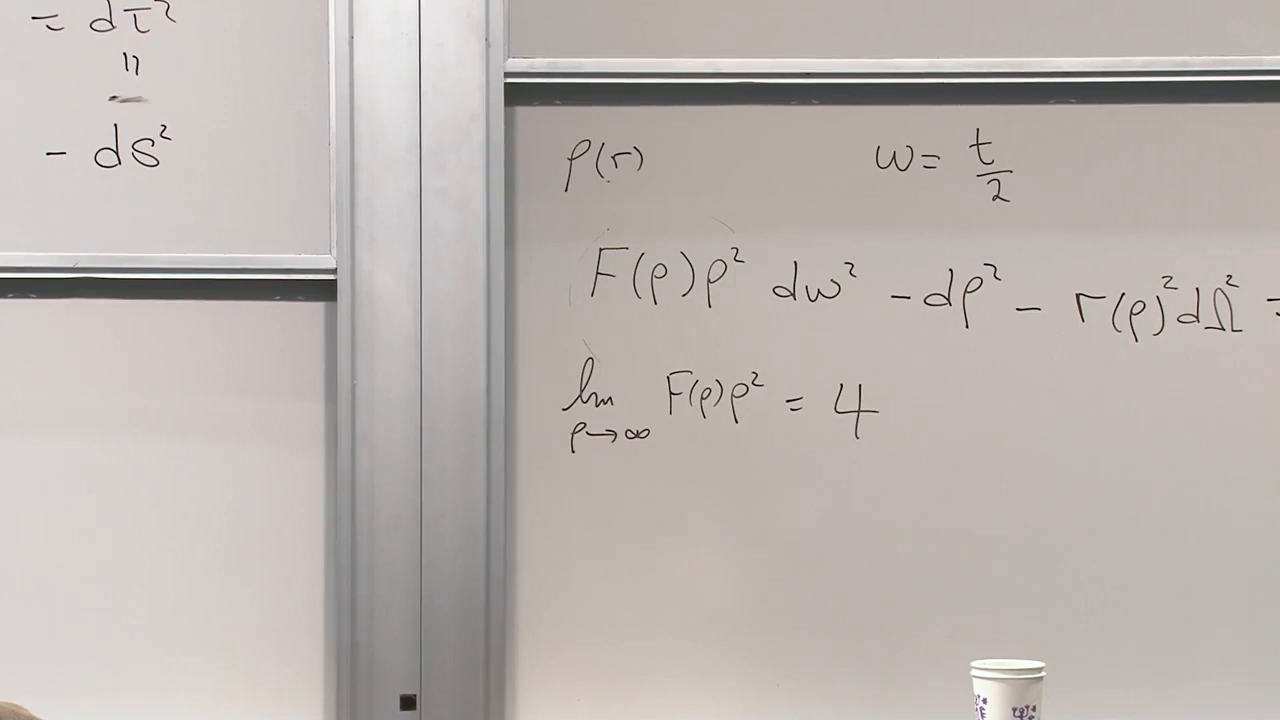
\includegraphics[width=0.90\textwidth]{lecture_07_figure_03.png}
\caption{Метрика в координатах \((\rho,\omega)\), ее асимптотический временной коэффициент и пригоризонтные пределы \(F\to1\) и
\(r=1+\rho^2/4+\cdots\).}
\lectureframe{00:37:30}
\end{figure}

\section{Плоское пространство-время, скрытое на горизонте}

Вблизи \(\rho=0\) радиально-временная часть
уравнения~\eqref{eq:l7-rho-metric} сводится к
\begin{equation}
d\tau_{\mathrm{radial}}^2
\simeq
\rho^2d\omega^2-d\rho^2.
\label{eq:l7-rindler-metric}
\end{equation}
Это плоское пространство-время Минковского в гиперболических полярных координатах. Введем
\begin{equation}
X=\rho\cosh\omega,
\qquad
T=\rho\sinh\omega.
\label{eq:l7-rindler-transform}
\end{equation}
Тогда
\begin{equation}
dT^2-dX^2
=
\rho^2d\omega^2-d\rho^2.
\label{eq:l7-minkowski-check}
\end{equation}
Кривые постоянного \(\rho\) удовлетворяют
\begin{equation}
X^2-T^2=\rho^2
\label{eq:l7-constant-rho}
\end{equation}
и являются гиперболами. Кривые постоянного \(\omega\) — это лучи, исходящие из начала координат. При \(\omega\to\infty\) эти лучи приближаются к светоподобной прямой \(T=X\). Следовательно, горизонт Шварцшильда, по-видимому отнесенный к бесконечному координатному времени, на регулярной диаграмме является обычной светоподобной прямой.

\begin{figure}[htbp]
\centering
\includegraphics[width=0.88\textwidth]{lecture_07_figure_06.png}
\caption{Завершенная геометрическая картина на доске: гиперболы постоянного \(\rho\),
лучи постоянного \(\omega\), светоподобный горизонт и область \(r<1\) над ним.}
\lectureframe{00:38:30}
\end{figure}

\begin{figure}[htbp]
\centering
\resizebox{0.96\linewidth}{!}{%
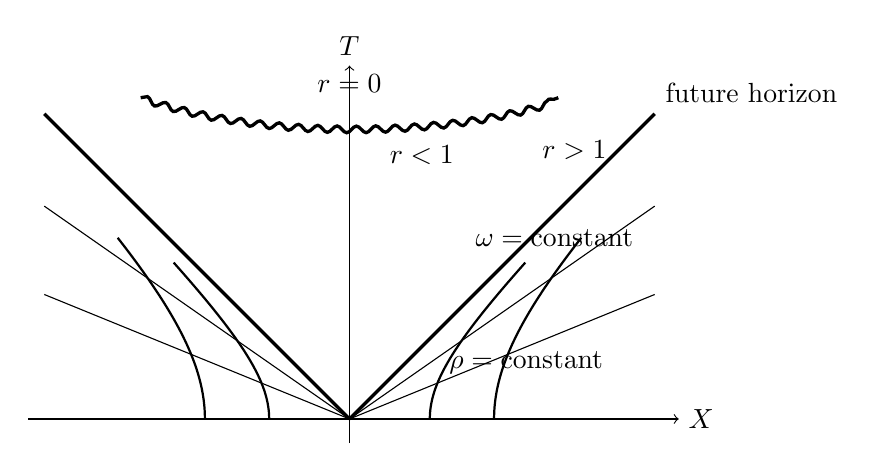
\begin{tikzpicture}[scale=1.02]
\draw[->] (-4.0,0) -- (4.1,0) node[right] {$X$};
\draw[->] (0,-0.3) -- (0,4.4) node[above] {$T$};
\draw[very thick] (0,0) -- (3.8,3.8)
  node[above right] {future horizon};
\draw[very thick] (0,0) -- (-3.8,3.8);
\draw[thick]
  plot[domain=0:1.42,samples=50]
  ({1.0*cosh(\x)},{1.0*sinh(\x)});
\draw[thick]
  plot[domain=0:1.05,samples=50]
  ({1.8*cosh(\x)},{1.8*sinh(\x)});
\draw[thick]
  plot[domain=0:1.42,samples=50]
  ({-1.0*cosh(\x)},{1.0*sinh(\x)});
\draw[thick]
  plot[domain=0:1.05,samples=50]
  ({-1.8*cosh(\x)},{1.8*sinh(\x)});
\draw[thin] (0,0) -- (3.8,1.55);
\draw[thin] (0,0) -- (3.8,2.65);
\draw[thin] (0,0) -- (-3.8,1.55);
\draw[thin] (0,0) -- (-3.8,2.65);
\draw[very thick,decorate,decoration={snake,amplitude=1.2pt,segment length=7pt}]
  (-2.6,4.0) .. controls (-1.2,3.5) and (1.2,3.5) .. (2.6,4.0);
\node at (0,4.18) {$r=0$};
\node at (2.2,0.7) {$\rho=\mathrm{constant}$};
\node at (2.55,2.25) {$\omega=\mathrm{constant}$};
\node at (0.9,3.28) {$r<1$};
\node at (2.8,3.35) {$r>1$};
\end{tikzpicture}
}
\caption{Ясная реконструкция причинной структуры. Горизонт является светоподобной прямой, тогда как сингулярность кривизны \(r=0\) есть будущая граница внутри черной дыры.}
\label{fig:l7-kruskal-clean}
\end{figure}

Предел при малом \(\rho\) не похож на предел малого радиуса в евклидовых полярных координатах. Малый евклидов круг стягивается к одной точке. Гипербола постоянного \(\rho\) приближается к целой светоподобной прямой. Поэтому \(\rho=0\) обозначает весь горизонт, а не только точку пересечения осей.

Внешнюю формулу можно аналитически продолжить в область \(r<1\). Вблизи горизонта, \(r-1\simeq\rho^2/4\), так что внутренней области формально соответствует
\(\rho^2<0\). Можно назвать \(\rho\) мнимой величиной, но чище использовать
\(\rho^2\), \(r\) или регулярные координаты \(T,X\). Внутри знаки коэффициентов при шварцшильдовских \(t\) и \(r\) меняются местами. Это не означает, что наручные часы физически превращаются в линейку. Это означает, что координаты Шварцшильда обменялись своим причинным характером.

\begin{classroomqa}
\audiencequestion{Что представляют собой горизонтальные гиперболы внутри горизонта и что представляют собой прямые лучи?}
\lecturerresponse{Гиперболические кривые — это линии постоянного \(r\), или, что то же самое, постоянного \(\rho^2\), продолженные в область \(r<1\). Лучи — это линии постоянного шварцшильдовского времени. Снаружи они образуют полезную координатную сетку; внутри те же обозначения нельзя принимать за физические траектории наблюдателей.
\lecturetimestamp{00:44:12--00:44:59}}
\end{classroomqa}

\begin{classroomqa}
\audiencequestion{Является ли вертикальное направление временной координатой и чью систему отсчета оно представляет?}
\lecturerresponse{Это регулярное временное направление на новой диаграмме пространства-времени, но это не сингулярное шварцшильдовское время \(t\). Диаграмма приспособлена к причинной структуре свободного падения. Наблюдатель, удерживаемый на фиксированном внешнем радиусе, движется по гиперболе и должен ускоряться; свободно падающий наблюдатель гладко пересекает светоподобный горизонт.
\lecturetimestamp{00:45:54--00:46:48}}
\end{classroomqa}

\begin{classroomqa}
\audiencequestion{Если внутри \(\rho^2<0\), то где явный множитель \(i\)?}
\lecturerresponse{Можно ввести мнимую \(\rho\), но это ничего не дает. Инвариантное содержание несут \(r\), \(\rho^2\) и вещественные регулярные координаты \(T,X\). Соотношение
\(r-1\simeq\rho^2/4\) — лишь пригоризонтное разложение.
\lecturetimestamp{00:52:35--00:53:00}}
\end{classroomqa}

На лекции эту регулярную диаграмму часто называют картиной Крускала. Строго говоря, точные координаты Крускала включают радиальный множитель, который сохраняет регулярность полной метрики Шварцшильда, тогда как уравнение~\eqref{eq:l7-rindler-transform} есть ее пригоризонтная форма. Причинный смысл тот же: горизонт гладок, но каждая направленная в будущее времениподобная или нулевая кривая внутри оканчивается на \(r=0\). Никакой сверхсветовой поворот не может вернуть ее обратно через горизонт.

\subsection{Как была понята координатная сингулярность}

Исторически было трудно увидеть гладкость горизонта, потому что исходные координаты Шварцшильда делают коэффициенты метрики на нем сингулярными на вид. Эддингтон, а позднее Финкельштейн, ввели координаты, пересекающие горизонт, и Финкельштейн распознал одностороннюю причинную границу. Крускал, чья легкость в обращении с преобразованиями координат пришла из физики плазмы, дал глобальную регулярную картину вечного решения.

Затем в лекции ненадолго останавливаются на Джоне Уилере, который помог сделать выражение «черная дыра» неизбежным. Эта пауза носит и личный, и исторический характер: Уилера помнят как мягкого и вдумчивого друга даже там, где политические оценки, включая оценки ядерного соперничества, резко расходились. Приводится забавная личная история, чтобы не сводить Уилера к карикатурному образу социально-конвенционального человека. Техническая тема возвращается в реплике: «у черных дыр нет волос». Возмущенная невращающаяся дыра быстро приходит к сферической симметрии; вращающаяся приходит к стационарной форме, задаваемой ее сохраняющимися параметрами. Это качественная версия идеи отсутствия волос, а не доказательство полной теоремы.

\section{Элис пересекает горизонт; Боб остается снаружи}

Максимально продолженная диаграмма содержит области, которые не возникают в простом пространстве-времени звезды, коллапсирующей из обычных начальных данных. Для мысленного эксперимента с наблюдателями мы используем только внешнюю область, горизонт будущего и внутренность черной дыры.

\begin{figure}[htbp]
\centering
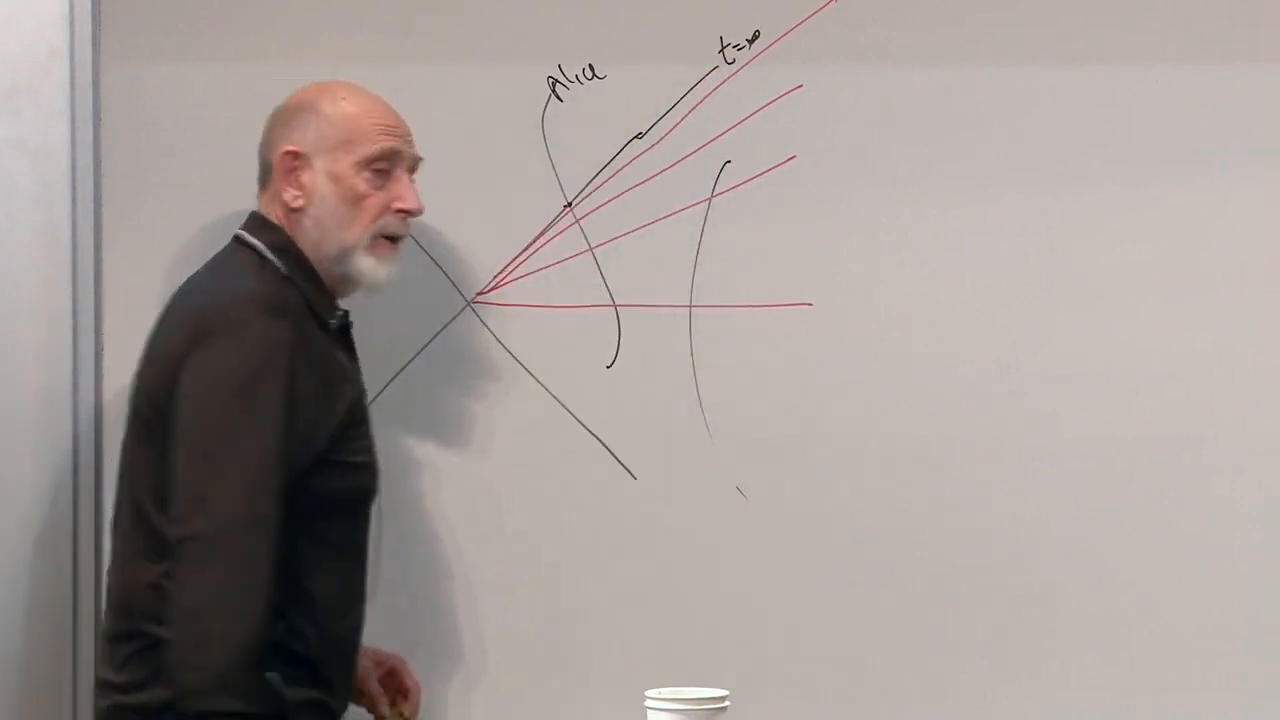
\includegraphics[width=0.84\textwidth]{lecture_07_figure_04.png}
\caption{Падающая мировая линия Элис и лучи постоянного шварцшильдовского времени. Предельный луч помечен \(t=\infty\).}
\lectureframe{00:54:54}
\end{figure}

Элис свободно падает. Ее мировая линия пересекает горизонт и достигает сингулярности за конечное собственное время. На горизонте с ее часами не происходит ничего особенного, если черная дыра достаточно велика и приливные силы там малы.

Боб, напротив, остается на фиксированном внешнем радиусе. Чтобы удерживаться на месте, требуется ускорение. Свет от более поздних точек траектории Элис приходит к нему со все большими задержками и со все большим красным смещением. В шварцшильдовом времени Элис приближается к \(t=\infty\), и Боб никогда не получает сигнала, испущенного после пересечения ею горизонта. Это утверждения о причинных сигналах и о разбиении внешней области на срезы, а не свидетельство существования материальной поверхности на горизонте.

\begin{classroomqa}
\audiencequestion{Если Боб видит, как Элис замедляется, должна ли Элис видеть, как Боб ускоряется?}
\lecturerresponse{Нет. Пока длится ее мировая линия, Элис продолжает получать от Боба обычные световые сигналы. На мировой линии Боба есть последнее событие, из которого сигнал может достичь ее, но оно является последним лишь потому, что затем Элис попадает в сингулярность. С самим Бобом не происходит ничего резкого. Наблюдение всегда обращено в прошлый световой конус, а две мировые линии находятся в асимметричном причинном отношении.
\lecturetimestamp{00:58:31--01:01:23}}
\end{classroomqa}

\begin{classroomqa}
\audiencequestion{Если Боб знает, что в его координатах Элис все еще близка к горизонту, может ли он спуститься, забрать ее и вернуться?}
\lecturerresponse{Мировая линия спасателя должна встретить Элис до того, как она пересечет горизонт событий. После этого события никакой направленный в будущее путь не может встретиться с ней и вернуться наружу. То, что шварцшильдовские срезы помещают это пересечение в \(t=\infty\), не означает, что Элис остается на какой-то материальной поверхности, с которой ее можно было бы забрать; это показывает, что такие срезы не задают глобального понятия «сейчас» по обе стороны горизонта.
\lecturetimestamp{01:01:24--01:02:12}}
\end{classroomqa}

\section{Чарли следует за Элис}

Пусть Чарли падает на небольшом расстоянии позади Элис. Тогда вблизи горизонта оба приблизительно инерциальны. Они могут обмениваться сигналами, вести двусторонний разговор или даже держаться за руки. Ни один из них не обнаруживает указателя, отмечающего горизонт. Контраст с Бобом — это не контраст между тремя поименованными людьми. Это контраст между свободным падением и ускоренной мировой линией, остающейся снаружи.

\begin{classroomqa}
\audiencequestion{Что видит Боб, если Элис падает первой, а Чарли следует за ней, словно баскетбольный мяч за кольцом?}
\lecturerresponse{Боб видит, как оба приближаются к горизонту. Элис, поскольку она впереди, первой выглядит все более замедлившейся и радиально сжатой. Чарли кажется все ближе и ближе позади нее, но в предельной внешней картине Боба никогда ее не догоняет. Это визуальное наслоение не описывает того, что ощущает ни один из падающих.
\lecturetimestamp{01:04:12--01:06:05}}
\end{classroomqa}

\begin{classroomqa}
\audiencequestion{Противоречит ли кажущееся уплощение приливной силе, которая должна растягивать падающего в радиальном направлении?}
\lecturerresponse{Это разные эффекты. Уплощение относится к шварцшильдовскому координатному описанию Боба. Приливное вытягивание — локальный эффект кривизны, который Элис и Чарли могут ощущать. В этом обсуждении с наблюдателями предполагается достаточно большая черная дыра или достаточно малые наблюдатели, так что приливным эффектом на горизонте можно пренебречь. Дыра с массой порядка солнечной, напротив, имела бы на горизонте очень сильные приливные силы, тогда как у сверхмассивной они могут быть слабыми.
\lecturetimestamp{01:06:07--01:08:18}}
\end{classroomqa}

\begin{classroomqa}
\audiencequestion{Видит ли Чарли, как Элис пересекает горизонт, пока он сам еще снаружи?}
\lecturerresponse{Постройте нулевой луч. Свет, испущенный Элис в момент пересечения, идет вдоль горизонта и достигает Чарли в тот момент, когда Чарли пересекает его. В этом событии он может вычислить, что увидел ее пересечение, хотя ни один из наблюдателей не встречает локальной метки. После этого он может видеть ее внутри. Если до пересечения он начнет ускоряться прочь и сумеет остаться снаружи, то никогда не увидит этого пересечения.
\lecturetimestamp{01:08:19--01:11:11}}
\end{classroomqa}

\begin{classroomqa}
\audiencequestion{Если Элис уже внутри, а Чарли снаружи, как можно сравнивать их более поздние радиусы и моменты пересечения?}
\lecturerresponse{Из фразы вроде «в одно и то же время» нельзя вывести никакого независимого от наблюдателя отношения одновременности. Элис видит Чарли на своем прошлом световом конусе и может увидеть его более позднее пересечение лишь тогда, когда сама находится глубже внутри. На вопрос отвечают конкретные мировые линии и нулевые лучи. Любую широкую экстраполяцию на множество далеко разнесенных падающих наблюдателей нужно проверять, рисуя их действительную причинную диаграмму, а не предполагая одно универсальное время пересечения.
\lecturetimestamp{01:11:14--01:12:31}}
\end{classroomqa}

В регулярных координатах вблизи горизонта траектория свободного падения почти представляет собой прямую линию. В полной геометрии Шварцшильда она не является в точности прямой, но это приближение становится хорошим вблизи большого горизонта со слабой кривизной.

\begin{classroomqa}
\audiencequestion{Может ли теория струн решить вопрос о том, что происходит в режиме квантовой гравитации внутри черной дыры?}
\lecturerresponse{Именно здесь предмет становится тонким. Вблизи сингулярности требуется квантовая теория гравитации, и теория струн является одним из возможных подходов, но соответствующие вопросы оставались активной и трудной областью исследований, а не были решены простым применением классической диаграммы.
\lecturetimestamp{01:13:04--01:13:38}}
\end{classroomqa}

\begin{classroomqa}
\audiencequestion{Что происходит с собственными часами Элис и с ее скоростью, когда она пересекает горизонт?}
\lecturerresponse{Ее часы продолжают тикать со своей обычной локальной скоростью хода и отсчитывают конечное собственное время. В своей мгновенной системе покоя она покоится; относительно локальной свободно падающей системы отсчета у нее обычная конечная скорость. Вблизи большого горизонта геометрия почти плоская, так что равные отметки собственного времени вдоль ее мировой линии остаются регулярными, пока кривизна не станет сильной вблизи сингулярности.
\lecturetimestamp{01:13:39--01:14:44}}
\end{classroomqa}

\begin{classroomqa}
\audiencequestion{Что если Боб ускоряется наружу, но недостаточно сильно, чтобы не провалиться через горизонт?}
\lecturerresponse{Тогда его мировая линия изгибается наружу, но все же пересекает горизонт. Если он пересекает его очень поздно, то может видеть Элис вскоре после ее пересечения, но оставшееся до сингулярности собственное время мало. Наклоны мировых линий на рисунке не являются откалиброванными линейками или часами; существенен причинный порядок, а не их нарисованные евклидовы длины.
\lecturetimestamp{01:14:47--01:16:31}}
\end{classroomqa}

Все эти выводы предполагают, что никакой сигнал не обгоняет свет. В лекции мимоходом шутят о тогдашних недавних сообщениях прессы о якобы сверхсветовых нейтрино в Италии; это намек на экспериментальную ошибку хронометража, а не на исключение из теории относительности. Сама причинная конструкция по-прежнему ограничена нулевыми линиями.

\begin{classroomqa}
\audiencequestion{Могут ли синхронизованные часы, которые несут Элис и Боб, решить вопрос, если Элис нырнет к горизонту и вернется?}
\lecturerresponse{Они могут сравнить часы, когда оказываются в одном и том же событии, но после того как их мировые линии расходятся, однозначной удаленной синхронизации нет, особенно когда один из них меняет движение. Нарисуйте обе мировые линии и обмениваемые нулевые лучи. Именно эта диаграмма дает операциональный ответ для любого заданного эксперимента.
\lecturetimestamp{01:17:34--01:18:25}}
\end{classroomqa}

\begin{figure}[htbp]
\centering
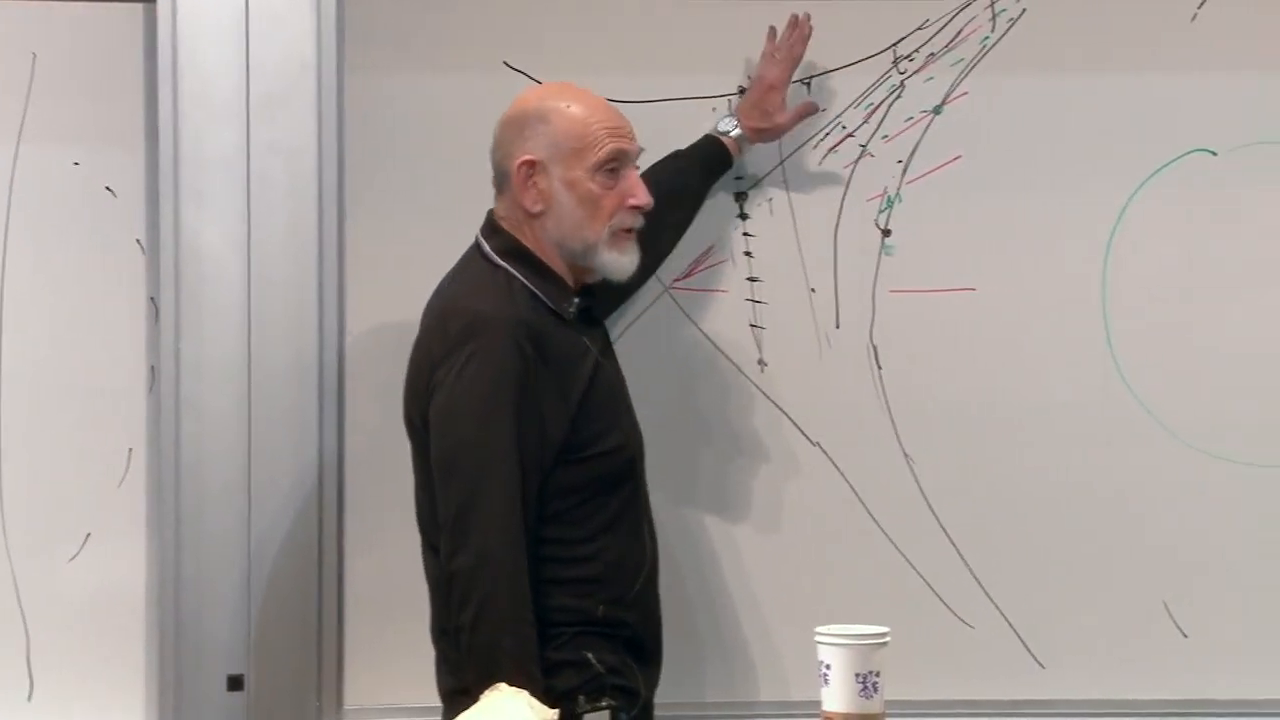
\includegraphics[width=0.86\textwidth]{lecture_07_figure_05.png}
\caption{Сводная причинная диаграмма, используемая для ответа на вопросы об Элис, Бобе и Чарли. Каждое наблюдение определяется проведением нулевого луча от наблюдаемого события к мировой линии наблюдателя.}
\lectureframe{01:18:12}
\end{figure}

\begin{figure}[htbp]
\centering
\resizebox{0.96\linewidth}{!}{%
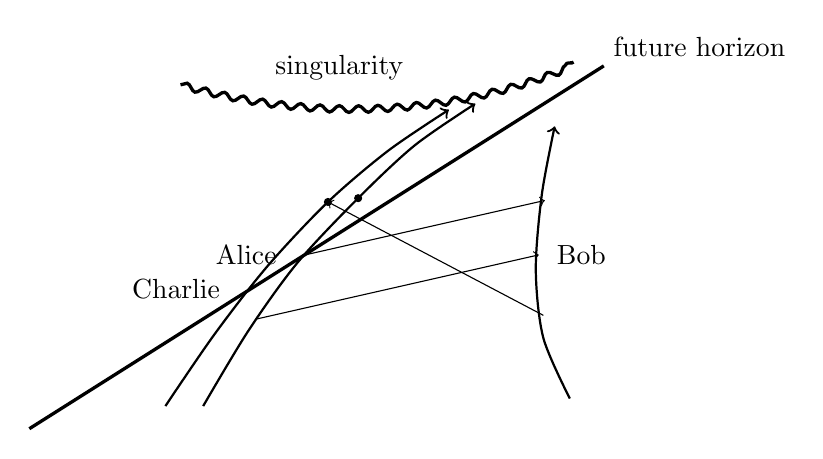
\begin{tikzpicture}[scale=0.96]
\draw[very thick] (-3.8,-0.3) -- (3.8,4.5);
\node[above right] at (3.8,4.5) {future horizon};
\draw[very thick,decorate,decoration={snake,amplitude=1.2pt,segment length=7pt}]
  (-1.8,4.25) .. controls (0.1,3.72) and (2.0,3.92) .. (3.4,4.55);
\node at (0.3,4.48) {singularity};
\draw[thick,->]
  plot[smooth] coordinates {(-1.5,0.0) (-0.9,1.0) (-0.25,1.9)
  (0.55,2.75) (1.3,3.45) (2.1,4.0)};
\node[left] at (-0.4,2.0) {Alice};
\draw[thick,->]
  plot[smooth] coordinates {(-2.0,0.0) (-1.35,0.95) (-0.65,1.85)
  (0.15,2.7) (0.95,3.38) (1.75,3.92)};
\node[left] at (-1.15,1.55) {Charlie};
\draw[thick,->]
  plot[smooth] coordinates {(3.35,0.1) (3.0,0.9) (2.9,1.8)
  (2.98,2.8) (3.15,3.7)};
\node[right] at (3.05,2.0) {Bob};
\draw[thin,->] (-0.8,1.15) -- (2.94,2.0);
\draw[thin,->] (-0.15,2.0) -- (3.02,2.72);
\draw[thin,->] (3.0,1.2) -- (0.15,2.7);
\draw[fill] (0.55,2.75) circle (1.3pt);
\draw[fill] (0.15,2.7) circle (1.3pt);
\end{tikzpicture}
}
\caption{Схематическая диаграмма наблюдателей. Внешние наблюдения Боба и взаимные наблюдения Элис и Чарли — это разные построения с нулевыми лучами, а не взаимные клише о часах.}
\label{fig:l7-observers-clean}
\end{figure}

\begin{classroomqa}
\audiencequestion{Видит ли Боб Алису бесконечно долго, и означает ли это, что в его реальности она никогда не умирает?}
\lecturerresponse{Боб получает ее сигналы на неограниченном интервале своего времени, но видит, как ход ее часов замедляется, стремясь к нулю, и получает лишь конечную последовательность ударов сердца, испущенных до того, как она его пересекла. Слово "реальность" скрывает различие между локальным событием и асимптотической регистрацией наблюдателя. На горизонте Алиса не сталкивается ни с какими остановившимися часами; запись Боба становится все более запаздывающей и все более красносмещенной.
\lecturetimestamp{01:18:32--01:20:59}}
\end{classroomqa}

\begin{classroomqa}
\audiencequestion{Видит ли Алиса внезапно всю старую материю, которая казалась застывшей на горизонте, как только она его пересекает?}
\lecturerresponse{Никакого внезапного прояснения не происходит. Пока она падает, прошлые световые конусы, посредством которых она видит более раннюю материю, непрерывно меняются. Она может заключить, что свет, достигающий ее сейчас, был испущен раньше и что материя пересекла его раньше нее. Взгляд Чарли на Алису дает тот же урок: ни одно из пересечений не создает локального разрыва и не обнаруживает скрытую груду стульев и динозавров.
\lecturetimestamp{01:21:02--01:23:48}}
\end{classroomqa}

\begin{classroomqa}
\audiencequestion{Существуют ли реалистичные симуляции того, что увидел бы падающий наблюдатель?}
\lecturerresponse{В лекции указывается на визуализации черных дыр Эндрю Хэмилтона. Они могут передавать сильную аберрацию и частотные сдвиги входящего света, хотя изображение может скорее дезориентировать, чем прояснять. Фраза «на горизонте ничего особенного» относится к локальной геометрии, а не к обычному на вид небу.
\lecturetimestamp{01:24:11--01:25:29}}
\end{classroomqa}

\section{От вечной черной дыры к растущей черной дыре}

Нижняя вершина максимально продолженной вечной диаграммы имеет мало прямого значения для черной дыры, образовавшейся при коллапсе звезды. В простой геометрии коллапса появляется лишь часть, содержащая внешнюю область, будущий горизонт и будущую внутреннюю область. Это различие становится существенным, когда допускается, что материя изменяет массу дыры.

\begin{classroomqa}
\audiencequestion{Какое физическое событие представлено нижней вершиной идеализированной диаграммы?}
\lecturerresponse{Для вечного математического решения это часть максимального продолжения. Черная дыра, образовавшаяся из коллапсирующей материи, не содержит всей этой нижней области. У ее горизонта есть история формирования, а это требует другой глобальной диаграммы и разбирается в следующей лекции.
\lecturetimestamp{01:25:59--01:26:52}}
\end{classroomqa}

Когда внутрь падает небольшое пробное тело, его обратным воздействием можно пренебречь, и фиксированная диаграмма Шварцшильда оказывается достаточной. Если падает существенная масса, масса черной дыры и радиус Шварцшильда увеличиваются:
\begin{equation}
r_{\mathrm S}=2GM,
\qquad
\Delta r_{\mathrm S}=2G\,\Delta M.
\label{eq:l7-growing-radius}
\end{equation}
Горизонт деформируется в сторону incoming объекта, горизонты соединяются, и искаженный общий горизонт быстро релаксирует. В невращающейся идеализации лекции конечным состоянием является немного большая сфера. Реальное слияние также излучает энергию в виде гравитационных волн и, как правило, оставляет после себя вращающуюся дыру.

\begin{classroomqa}
\audiencequestion{Если при падении массы горизонт растет, движется ли он наружу, чтобы встретить материю, которая казалась застывшей у старого горизонта?}
\lecturerresponse{Для достаточно массивного падающего объекта картина пробной частицы уже неприменима. Горизонт деформируется, соединяется с захваченной областью падающего объекта и релаксирует к большему стационарному горизонту. Точное положение горизонта событий определяется глобально и может простираться в область, предшествующую приходу падающей материи. В лекции полное построение намеренно отложено до следующего занятия.
\lecturetimestamp{01:26:55--01:29:05}}
\end{classroomqa}

\begin{classroomqa}
\audiencequestion{Почему астрономы могут видеть вспышки, если, как говорится, материи требуется бесконечное время Шварцшильда, чтобы достичь горизонта?}
\lecturerresponse{Яркое излучение исходит не от самого горизонта. Газ в аккреционном потоке или диске сталкивается и нагревается вне горизонта, в том числе вблизи фотонных орбит. Эта внешняя плазма может испускать свет, достигающий нас. Пустая геометрия Шварцшильда изолирует причинную задачу, но не является полной моделью астрофизической среды.
\lecturetimestamp{01:29:07--01:30:22}}
\end{classroomqa}

Характерное время релаксации задается временем прохождения света:
\begin{equation}
t_{\mathrm{cross}}\sim\frac{r_{\mathrm S}}{c},
\qquad
t_{\mathrm{relax}}\sim
\text{a few to a few tens of }t_{\mathrm{cross}}.
\label{eq:l7-relaxation-scale}
\end{equation}
В лекции \(10^{-5}\,\mathrm{s}\) оценивается как время пересечения для дыры километрового масштаба, а примерно \(10^{-3}\,\mathrm{s}\) — как время, за которое после небольшого слияния она становится почти стационарной. Для дыры с массой в миллиард солнечных масс соответствующее время измеряется минутами или часами. Это масштабные оценки, а не точные расчеты слияния. Суть в геометрической последовательности: гантель, арахис, почти сферическая форма, стационарное состояние.

\begin{classroomqa}
\audiencequestion{Как быстро устанавливается искаженный горизонт или горизонт сразу после слияния?}
\lecturerresponse{На временном масштабе, не намного большем, чем нужно свету, чтобы пересечь дыру. Поскольку каждая длина и каждое время масштабируются с \(r_{\mathrm S}\), малые дыры устанавливаются за доли секунды, а сверхмассивные — за гораздо более длительные интервалы времени. Утверждение об отсутствии волос описывает стационарный конечный результат; переходная деформация уносит энергию в виде гравитационного излучения.
\lecturetimestamp{01:30:26--01:33:18}}
\end{classroomqa}

\begin{classroomqa}
\audiencequestion{Что видит Боб, если ранее упавшая материя находится между старым и новым горизонтом, пока внутрь падает еще одно массивное тело?}
\lecturerresponse{На этот вопрос нельзя последовательно ответить, просто сшив вместе две статические диаграммы Шварцшильда. Нужно решить или построить зависящую от времени геометрию коллапса и определить положение ее глобального горизонта. Лекция сохраняет этот вопрос и прямо откладывает ответ до следующей недели, где предметом будет формирование горизонта.
\lecturetimestamp{01:33:20--01:35:41}}
\end{classroomqa}

\section{Что меняется при изменении масштаба?}

Безразмерная диаграмма не меняется при изменении \(r_{\mathrm S}\). А вот физический смысл изображенного интервала меняется:
\begin{equation}
d\tau_{\mathrm{physical}}^2
=
r_{\mathrm S}^2\,d\hat{\tau}^2,
\qquad
\ell_{\mathrm{physical}}
=
r_{\mathrm S}\,\hat{\ell}.
\label{eq:l7-scale-restoration}
\end{equation}
Безразмерное расстояние, которое для дыры километрового масштаба соответствует половине километра, для дыры в миллиард раз большей соответствует примерно половине миллиарда километров. Здесь снова полезна аналогия с одинаково нарисованными сферами: форма не меняется, тогда как число метровых линеек, представленных отрезком, масштабируется с радиусом.

\begin{classroomqa}
\audiencequestion{Как меняется причинная диаграмма при изменении радиуса Шварцшильда?}
\lecturerresponse{После того как радиус вынесен в масштаб, она не меняется. Каждая физическая длина и каждое физическое время, приписываемые диаграмме, умножаются на \(r_{\mathrm S}\), тогда как кривизна в соответствующих безразмерных точках умножается на \(r_{\mathrm S}^{-2}\).
\lecturetimestamp{01:35:41--01:38:10}}
\end{classroomqa}

\begin{classroomqa}
\audiencequestion{Меняется ли причинный вывод, если Боб движется по орбите, а не зависает в одном угловом положении?}
\lecturerresponse{Подробные красные смещения и направления прихода становятся сложнее, но причинная отделенность горизонта не меняется. Ни одна времениподобная орбита во внешней области не получает сигнала, испущенного изнутри горизонта.
\lecturetimestamp{01:38:12--01:38:26}}
\end{classroomqa}

\begin{classroomqa}
\audiencequestion{Поскольку внутри сферической оболочки гравитация исчезает, исчезает ли она и внутри горизонта, потому что масса черной дыры распределена по этой поверхности?}
\lecturerresponse{Нет. Горизонт событий — не материальная оболочка, несущая массу. Поэтому ньютоновская теорема об оболочке к нему не применяется. В лекции статическое внешнее решение сравнивается с точечным источником в сингулярности кривизны, но материя, продолжающая падать во время формирования, требует зависящей от времени геометрии, рассмотрение которой отложено до следующей лекции.
\lecturetimestamp{01:38:28--01:40:41}}
\end{classroomqa}

\section{Вращение и радиальная геометрия}

Угловой момент сохраняется при коллапсе. У вращающейся черной дыры внешняя геометрия отличается от шварцшильдовской: ее стационарное решение — решение Керра, вращение искажает геометрию горизонта, а увлечение инерциальных систем поворачивает инерциальные направления вокруг дыры. В принципе угловой момент измеряют по этим внешним гравитационным эффектам. Материя, обладающая угловым моментом, не теряет его просто потому, что пересекает горизонт.

\begin{classroomqa}
\audiencequestion{Может ли черная дыра иметь измеримый угловой момент, и меняет ли вращение гравитацию вне нее?}
\lecturerresponse{Да. Угловой момент остается сохраняющимся параметром, деформирует стационарную геометрию и вызывает увлечение инерциальных систем. Горизонт уже не является простым сферическим горизонтом Шварцшильда. В лекции это искажение качественно сравнивается со сплюснутой формой Земли, при этом отмечается, что полное вращающееся решение существенно сложнее.
\lecturetimestamp{01:40:45--01:42:36}}
\end{classroomqa}

\begin{classroomqa}
\audiencequestion{Означает ли соотношение между \(r\) и собственным расстоянием \(\rho\), что гравитация сжимает пространство?}
\lecturerresponse{Собственное радиальное расстояние \(\rho\) удовлетворяет соотношению
\begin{equation*}
\frac{d\rho}{dr}=\sqrt{\frac{r}{r-1}}>1
\end{equation*}
вне единичного горизонта. Поэтому данному координатному приращению \(dr\) вблизи горизонта соответствует больший собственный радиальный интервал. Говорить, что пространство сжато или растянуто, зависит от того, какие координатные интервалы сравниваются. Инвариантным утверждением является само соотношение для собственного расстояния.
\lecturetimestamp{01:42:36--01:43:20}}
\end{classroomqa}

\section{Заключительные вопросы}

\begin{classroomqa}
\audiencequestion{С точки зрения Боба ход часов Алисы стремится к остановке. С точки зрения Алисы, приходит ли к концу пространство или время Боба?}
\lecturerresponse{Нет. Алиса видит обычные сигналы от последовательных событий на мировой линии Боба, пока не заканчивается ее собственная мировая линия. Более поздние события Боба она не видит потому, что на ее мировой линии не существует более поздней точки, а не потому, что Боб или его пространство исчезают. В этих регулярных причинных координатах радиальные светоподобные лучи изображаются прямыми; то, что в другой системе координат они выглядят как искривленные траектории, не меняет того, какие события они соединяют.
\lecturetimestamp{01:43:21--01:45:20}}
\end{classroomqa}

Общая теория относительности ставит две взаимодополняющие задачи. Задав метрику, можно проследить геодезические и светоподобные лучи, чтобы определить, что измеряют наблюдатели. Задав распределение материи, нужно решить уравнения Эйнштейна, чтобы найти метрику. Этой лекции была посвящена первая задача. Вторая обычно труднее, хотя симметричный коллапс дает примеры, поддающиеся рассмотрению.

\begin{classroomqa}
\audiencequestion{Что происходит с горизонтом и сингулярностью испаряющейся черной дыры?}
\lecturerresponse{В лекции дается схематическая картина, в которой горизонт сжимается и встречается с конечной точкой сингулярной области. Испарение — это полуклассический квантовый процесс, и конечная стадия планковского масштаба не определяется классической диаграммой Шварцшильда. Поэтому эту схему с уменьшающимся горизонтом следует понимать как качественный предварительный набросок, а не как полную квантовую геометрию.
\lecturetimestamp{01:46:04--01:46:32}}
\end{classroomqa}

Почти каждая астрофизическая черная дыра должна вращаться. Звезды уже обладают моментом импульса, и коллапс увеличивает их угловую скорость знакомым образом, как у фигуриста, прижимающего руки к телу. Сингулярная структура черной дыры Керра — не та шварцшильдовская поверхность \(r=0\), которая изображена здесь, и ее не следует описывать так, будто материя буквально вращается с бесконечной линейной скоростью.

\begin{classroomqa}
\audiencequestion{Часто ли встречаются невращающиеся макроскопические черные дыры, и сколько существует черных дыр?}
\lecturerresponse{Строго нулевой момент импульса был бы исключительной идеализацией. На лекции приводится лишь аудиторная прикидка порядка величины для их космического числа: где-то между числом галактик и числом звезд и, возможно, порядка \(10^{15}\). Это оценка, данная в лекции, а не результат измеренного подсчета. Надежный вывод состоит в том, что коллапс, вообще говоря, сохраняет и усиливает некоторый момент импульса.
\lecturetimestamp{01:46:32--01:48:42}}
\end{classroomqa}

\begin{classroomqa}
\audiencequestion{Черные дыры образуются из уже существующей материи или возникают в результате квантового процесса?}
\lecturerresponse{Обычные астрофизические черные дыры образуются при коллапсе уже существующей звездной материи. Термоядерное горение и направленный наружу поток энергии помогают поддерживать звезду. Когда топливо исчерпывается, остаток сжимается. В зависимости от своей массы и доступной опоры за счет давления он может стать белым карликом, нейтронной звездой или, если никакая опора давлением не может остановить коллапс, уйти внутрь собственного шварцшильдовского радиуса и образовать черную дыру.
\lecturetimestamp{01:48:43--01:50:23}}
\end{classroomqa}

\begin{classroomqa}
\audiencequestion{Могли бы образовываться микроскопические черные дыры, и чем определялись бы их время жизни и минимальный размер?}
\lecturerresponse{Эта часть носит спекулятивный характер. Испарение Хокинга идет быстрее при меньшей массе, причем время жизни масштабируется примерно как \(M^3\). В лекции для дыры, время жизни которой могло бы быть космологическим, используется сравнение с массой горы; эта численная аналогия лишь грубая. Возможными механизмами образования могут быть сильные флуктуации плотности в ранней Вселенной или достаточно энергичные столкновения. Черная дыра с массой порядка планковской, примерно \(10^{-5}\,\mathrm{g}\), отмечает масштаб, на котором классическому геометрическому описанию уже нельзя доверять. Достижение такой энергии в обычном ускорителе потребовало бы неправдоподобно большой установки при прямой экстраполяции, хотя такое образование в принципе возможно.
\lecturetimestamp{01:50:23--01:53:31}}
\end{classroomqa}

\begin{classroomqa}
\audiencequestion{Дойдет ли курс до космологии, темной материи, темной энергии, энтропии и гравитационных волн?}
\lecturerresponse{Космологические приложения и, возможно, гравитационные волны еще могут стать темами для более позднего рассмотрения. Энтропия черных дыр отложена за пределы квартала. Лекция завершается признанием, что в тот вечер удалось пройти лишь около четверти запланированного материала: важнее тщательно разбирать вопросы, чем поспешно пробегать план.
\lecturetimestamp{01:53:33--01:54:38}}
\end{classroomqa}

Операционное правило выдерживает любой вопрос, возникающий в аудитории. Задайте мировые линии, проведите светоподобные лучи и укажите события, которые они соединяют. Горизонт — не место, где нарушается локальная физика; это граница, за которой всякий направленный в будущее сигнал остается внутри. На следующей лекции вместо вечного фона будет рассматриваться коллапсирующий источник, и будет показано, как формируется эта граница.